\documentclass[11pt]{article}

\usepackage[margin=0.85in]{geometry}
\usepackage[T1]{fontenc}
\usepackage[utf8]{inputenc}
\usepackage{lmodern}
\usepackage{amsmath,amssymb,mathtools}
\usepackage{booktabs}
\usepackage{array}
\usepackage{enumitem}
\usepackage{longtable}
\usepackage{xcolor}
\usepackage{hyperref}
\usepackage{tikz}
\usepackage[most]{tcolorbox}
\usetikzlibrary{arrows.meta,positioning,calc,shapes.geometric}

\hypersetup{
  colorlinks=true,
  linkcolor=blue!55!black,
  urlcolor=blue!55!black,
  citecolor=blue!55!black
}

\setlist[itemize]{topsep=2pt,itemsep=2pt,leftmargin=*}
\setlist[enumerate]{topsep=2pt,itemsep=2pt,leftmargin=*}
\renewcommand{\arraystretch}{1.16}

\definecolor{MSBlue}{RGB}{20,77,120}
\definecolor{SoftBlue}{RGB}{236,245,255}
\definecolor{SoftGreen}{RGB}{236,248,238}
\definecolor{SoftYellow}{RGB}{255,250,232}
\definecolor{SoftRed}{RGB}{255,241,241}

\newtcolorbox{keybox}[1]{
  enhanced,
  breakable,
  colback=SoftBlue,
  colframe=MSBlue,
  title=\textbf{#1},
  arc=2mm,
  boxrule=0.6pt
}

\newtcolorbox{answerbox}[1]{
  enhanced,
  breakable,
  colback=SoftGreen,
  colframe=green!40!black,
  title=\textbf{#1},
  arc=2mm,
  boxrule=0.6pt
}

\newtcolorbox{examplebox}[1]{
  enhanced,
  breakable,
  colback=SoftYellow,
  colframe=orange!65!black,
  title=\textbf{#1},
  arc=2mm,
  boxrule=0.6pt
}

\newtcolorbox{warningbox}[1]{
  enhanced,
  breakable,
  colback=SoftRed,
  colframe=red!55!black,
  title=\textbf{#1},
  arc=2mm,
  boxrule=0.6pt
}

\newcommand{\Hz}{\mathrm{Hz}}
\newcommand{\V}{\mathrm{V}}
\newcommand{\A}{\mathrm{A}}
\newcommand{\W}{\mathrm{W}}
\newcommand{\kW}{\mathrm{kW}}
\newcommand{\kVA}{\mathrm{kVA}}
\newcommand{\pu}{\mathrm{pu}}

\title{\textbf{Mainspring Interview Preparation Guide}\\
\large Inverter Systems Integration Engineer -- Electrical (Menlo Park, CA)}
\author{Role-Specific Technical and Behavioral Notes}
\date{\today}

\begin{document}
\maketitle

\begin{abstract}
This guide is tailored to an electrical systems-integration role focused on
industrial grid-interactive inverters that interface generation assets to the
customer grid. It prioritizes system architecture, lab validation, parameter
tuning, field troubleshooting, standards compliance (IEEE 1547, UL 1741), and
cross-functional execution through the full product lifecycle.
\end{abstract}

\begin{keybox}{Core interview message}
``I specialize in making power conversion hardware behave predictably in real
grids. I can select and tune OTS inverters, design evidence-based validation
tests, and close the loop from lab characterization to field root-cause
resolution while maintaining safety and compliance.''
\end{keybox}

\tableofcontents
\newpage

\section{Role Decomposition: What You Are Being Hired To Do}

This role is fundamentally a \textbf{systems-integration authority} position.
You are expected to connect hardware capability, control behavior, grid
interconnection requirements, and field reliability into one coherent
engineering workflow.

\begin{itemize}
  \item Own system-level integration of high-power inverters, rather than printed circuit board (PCB) level converter design.
  \item Configure and validate both grid-following (GFL) and grid-forming (GFM) behavior.
  \item Lead technical decisions for off-the-shelf (OTS) inverter selection and sizing.
  \item Build and execute low-voltage ride-through (LVRT), frequency-response, and power-quality test campaigns.
  \item Diagnose failures with waveform-first, hypothesis-driven troubleshooting.
  \item Translate standards into concrete design limits, settings, and pass/fail criteria.
\end{itemize}

\subsection{Acronyms and terms used in this guide}
\begin{longtable}{p{0.19\linewidth}p{0.75\linewidth}}
\toprule
Term & Meaning \\
\midrule
AC & Alternating current \\
CAN & Controller Area Network \\
DC & Direct current \\
EMI & Electromagnetic interference \\
GFL & Grid-following inverter control mode \\
GFM & Grid-forming inverter control mode \\
HIL & Hardware-in-the-loop validation setup \\
IEEE & Institute of Electrical and Electronics Engineers \\
LVRT & Low-voltage ride-through \\
Modbus RTU & Modbus Remote Terminal Unit (serial) \\
Modbus TCP & Modbus over Transmission Control Protocol network transport \\
NEC & National Electrical Code (NFPA 70) \\
OCPD & Overcurrent protective device \\
OTS & Off-the-shelf equipment \\
PCB & Printed circuit board \\
PF & Power factor \\
PLL & Phase-locked loop \\
RCA & Root-cause analysis \\
RMS & Root-mean-square \\
SCR & Short-circuit ratio \\
STAR & Situation, Task, Action, Result behavioral response format \\
UL & Underwriters Laboratories \\
\bottomrule
\end{longtable}

\subsection{Role outcomes interviewers care about}
\begin{table}[h]
\centering
\begin{tabular}{p{0.25\linewidth}p{0.32\linewidth}p{0.33\linewidth}}
\toprule
Workstream & Typical deliverable & Interview evidence you should present \\
\midrule
Architecture and integration & Interface control settings, protection boundaries, commissioning profile & Tradeoff story where stability and compliance both improved \\
Lab validation & Test matrix, waveform package, pass/fail report & One campaign with quantified before/after tuning result \\
Field reliability & RCA memo, corrective action plan, regression closure & One field issue closed end-to-end with measurable uptime impact \\
Cross-functional execution & Design review decisions and change records & Example of influencing controls, mechanical, and test teams together \\
\bottomrule
\end{tabular}
\end{table}

\section{Technical Foundations You Must Communicate Clearly}

\subsection{Grid-following versus grid-forming in practical terms}
\begin{itemize}
  \item GFL inverters synchronize to an existing grid voltage and frequency reference, usually via a PLL.
  \item GFM inverters establish voltage and frequency references and can support weak-grid or islanded operation.
  \item Integration risk appears at mode transitions, low SCR, control-loop interaction, and protection coordination.
\end{itemize}

\begin{table}[h]
\centering
\begin{tabular}{p{0.23\linewidth}p{0.34\linewidth}p{0.34\linewidth}}
\toprule
Dimension & Grid-following (GFL) & Grid-forming (GFM) \\
\midrule
Reference source & Tracks external grid phase/frequency via PLL & Establishes internal voltage/frequency reference \\
Weak-grid behavior & Sensitive to low SCR and PLL tuning & Typically stronger support if droop and virtual impedance are tuned \\
Islanding capability & Usually limited without external source & Can support intentional island operation if certified and configured \\
Protection interaction & Trip-prone when phase/frequency estimates become noisy & Can still trip if current limit and protection transitions are poorly tuned \\
Primary tuning focus & PLL bandwidth, current-loop damping & Droop slopes, virtual impedance, current limiting and anti-windup \\
\bottomrule
\end{tabular}
\end{table}

\begin{answerbox}{Interview-ready one-liner}
``Grid-following control is excellent when a stiff grid exists, but for weak
grids and ride-through resilience, grid-forming behavior with well-damped outer
loops and correctly tuned current limits is often the difference between stable
operation and oscillatory trips.''
\end{answerbox}

\subsection{Short-circuit ratio and weak-grid stability}
Common shorthand:
\[
\mathrm{SCR} = \frac{S_{\mathrm{sc}}}{S_{\mathrm{inv,rated}}}.
\]
where \(S_{\mathrm{sc}}\) is available short-circuit apparent power at the
point of interconnection and \(S_{\mathrm{inv,rated}}\) is inverter nameplate
apparent power. As SCR decreases, PLL-based controls and fast current loops can
become less tolerant of delays and phase lag.

Discuss mitigation in a structured way:
\begin{itemize}
  \item Lower PLL bandwidth for GFL systems.
  \item Adjust virtual impedance and droop gains for GFM systems.
  \item Validate with impedance-scan or step-response style tests in a controlled lab setup.
  \item Confirm no adverse interaction with plant-level controllers and utility voltage-regulation equipment.
\end{itemize}

\begin{examplebox}{Strong technical framing in interviews}
``I use SCR as a screening metric, not as the only metric. Then I validate
control robustness with measured step responses, harmonic sensitivity checks,
and coordinated protection behavior under degraded grid conditions.''
\end{examplebox}

\subsection{Real and reactive control framing}
For AC-side dispatch and support:
\[
P = 3 V_{\phi} I_{\phi} \cos\theta, \quad Q = 3 V_{\phi} I_{\phi} \sin\theta.
\]
In interview discussion, tie this to settings and constraints:
\begin{itemize}
  \item Volt-var curves for voltage support.
  \item Frequency-watt or droop response for frequency events.
  \item Current limits and anti-windup strategy under faults.
  \item Priority logic (for example, reactive priority versus active-power priority) during voltage disturbances.
\end{itemize}

\begin{table}[h]
\centering
\begin{tabular}{p{0.26\linewidth}p{0.31\linewidth}p{0.34\linewidth}}
\toprule
Control function & Main objective & Integration watch-out \\
\midrule
Volt-var & Local voltage support via reactive power command & Interaction with feeder regulator deadbands \\
Frequency-watt & Frequency stabilization using active-power droop & Energy-source limits and ramp-rate boundaries \\
Current limiting & Protect semiconductor and magnetic components & Nonlinear transition behavior that can excite oscillation \\
Ride-through logic & Maintain service through disturbances & Nuisance trips from poorly coordinated timers/thresholds \\
\bottomrule
\end{tabular}
\end{table}

\section{OTS Inverter Selection and Sizing Framework}

\begin{keybox}{Selection checklist}
\begin{enumerate}
  \item Electrical envelope: DC input range, AC nominal voltage, fault current behavior.
  \item Overload and transient capability: peak current duration, thermal derating.
  \item Control features: GFM/GFL support, droop modes, black-start/islanding capabilities.
  \item Grid-code feature set: IEEE 1547 functions, ride-through programmability.
  \item Communications: Modbus TCP/RTU, CAN, SunSpec points map quality.
  \item Serviceability: diagnostics, event logs, firmware maturity, vendor support cadence.
\end{enumerate}
\end{keybox}

\subsection{Comparing candidate inverter platforms}
\begin{table}[h]
\centering
\begin{tabular}{p{0.2\linewidth}p{0.25\linewidth}p{0.25\linewidth}p{0.2\linewidth}}
\toprule
Criterion & Candidate A & Candidate B & Decision cue \\
\midrule
Continuous \(\kVA\) and overload & Strong continuous, modest overload & Moderate continuous, strong short overload & Match to duty cycle and fault support expectation \\
GFM maturity & Basic droop only & Advanced droop plus virtual impedance & Favor higher control maturity for weak-grid projects \\
Diagnostics and logs & Coarse event logs & High-resolution event and waveform logs & Faster RCA favors richer diagnostics \\
Communications profile & Vendor-specific mapping & SunSpec-aligned mapping & Interoperability favors standardized mapping \\
Service ecosystem & Slow firmware turnaround & Responsive field support & Fleet reliability favors faster support cycle \\
\bottomrule
\end{tabular}
\end{table}

\subsection{Quick sizing equations for interview whiteboard use}
Use this sequence on a whiteboard so your logic is easy to follow:

\begin{enumerate}
  \item Define site and dispatch assumptions: \(V_{LL}\), target \(P\), required power factor range, inverter efficiency \(\eta\), ambient derating, and required reactive support profile.
  \item Convert required \(P\) and \(Q\) into apparent power \(S\).
  \item Size AC current and compare against continuous and short-duration current limits.
  \item Apply engineering margin for thermal derating, manufacturing spread, and future firmware control changes.
\end{enumerate}

\subsubsection*{Step 1: AC current from real-power target}
\[
I_{\mathrm{line}} \approx \frac{P}{\sqrt{3}V_{LL}\,\eta\,\mathrm{pf}}.
\]
This gives a first-pass continuous current estimate for conductor, breaker, and
thermal checks. Mention in interview that this is a planning equation and that
final values should use manufacturer current limits and protection coordination.

\subsubsection*{Step 2: Apparent power and reactive headroom}
\[
S = \sqrt{P^2 + Q^2}, \qquad S \le S_{\mathrm{rated}}.
\]
Useful alternate forms:
\[
\mathrm{pf} = \frac{P}{S}, \qquad Q = P\tan(\cos^{-1}(\mathrm{pf})).
\]
If the interconnection requires non-unity PF operation, explain that inverter
real-power dispatch may be intentionally capped to preserve \(Q\) capacity.

\subsubsection*{Step 3: Margining for real projects}
A common interview-safe expression is:
\[
S_{\mathrm{required}} = \frac{\sqrt{P^2 + Q^2}}{k_{\mathrm{derate}}},
\]
where \(k_{\mathrm{derate}} < 1\) captures temperature, altitude, and enclosure
cooling effects. If \(k_{\mathrm{derate}} = 0.9\), you need roughly 11\% more
nameplate \(S\) than the nominal operating point.

\subsubsection*{Step 4: DC-side sanity check}
For a quick consistency check:
\[
P_{\mathrm{dc}} \approx \frac{P_{\mathrm{ac}}}{\eta}, \qquad
I_{\mathrm{dc}} \approx \frac{P_{\mathrm{dc}}}{V_{\mathrm{dc}}}.
\]
Then verify that the DC source, bus voltage window, and ripple-current limits
remain valid through transients and fault ride-through events.

\begin{examplebox}{Worked whiteboard example}
Assume a \(480~\mathrm{V}_{LL}\) system, target \(P=500~\kW\),
\(\eta=0.97\), and minimum operating power factor \(\mathrm{pf}=0.9\).

1) Continuous line current:
\[
I_{\mathrm{line}} \approx
\frac{500\times 10^3}{\sqrt{3}\cdot 480 \cdot 0.97 \cdot 0.9}
\approx 689~\mathrm{A}.
\]

2) Apparent power at \(\mathrm{pf}=0.9\):
\[
S = \frac{P}{\mathrm{pf}} = \frac{500}{0.9} \approx 556~\kVA.
\]

3) Reactive power capability at that point:
\[
Q = \sqrt{S^2 - P^2} \approx 241~\mathrm{kVAr}.
\]

4) If thermal derating factor is \(k_{\mathrm{derate}}=0.92\):
\[
S_{\mathrm{required}} \approx \frac{556}{0.92} \approx 604~\kVA.
\]
So a 600 kVA class inverter is likely tight; a larger rating gives practical
margin for high-ambient operation and dynamic support obligations.
\end{examplebox}

\begin{warningbox}{Sizing pitfalls interviewers listen for}
\begin{itemize}
  \item Using only \(P\)-rating and forgetting reactive support commitments.
  \item Ignoring derating at site ambient and enclosure conditions.
  \item Assuming continuous current equals transient/fault-current capability.
  \item Missing cable, OCPD, and transformer constraints while focusing only on inverter datasheet limits.
\end{itemize}
\end{warningbox}

\subsection{Interview whiteboard sequence that looks senior}
\begin{enumerate}
  \item State assumptions first: voltage level, ambient temperature, PF envelope, utility requirements.
  \item Show equations second: current, \(S\), and derating-adjusted requirement.
  \item Convert equations to selection implications: minimum \(\kVA\), current rating, and control-feature requirements.
  \item End with validation plan: how you will verify the sizing decision in lab and in commissioning.
\end{enumerate}

\section{Lab Validation Strategy (High Signal-to-Noise Testing)}

\subsection{Recommended test pyramid}
\begin{enumerate}
  \item Bench parameter sanity and comms verification.
  \item Hardware-in-the-loop or grid emulator dynamic tests.
  \item Full-power integrated tests with representative source/load dynamics.
  \item Stress tests for edge cases: weak grid, fast ramps, voltage dips, phase steps.
\end{enumerate}

\begin{table}[h]
\centering
\begin{tabular}{p{0.2\linewidth}p{0.25\linewidth}p{0.23\linewidth}p{0.24\linewidth}}
\toprule
Layer & Typical objective & Main instruments & Exit criterion \\
\midrule
Bench bring-up & Confirm settings and interfaces & Scope, protocol sniffer, power analyzer & Stable command/telemetry and no basic alarms \\
HIL or emulator & Validate control dynamics safely & Grid emulator, recorder, event logger & Damped response to steps and disturbances \\
Integrated full power & Verify thermal/electrical performance & Calibrated analyzers, thermal sensors & Meets continuous duty and protection expectations \\
Edge-case stress & Reveal hidden instability margins & Disturbance scripts and fault playback & No unstable oscillation or nuisance trips in required envelope \\
\bottomrule
\end{tabular}
\end{table}

\begin{center}
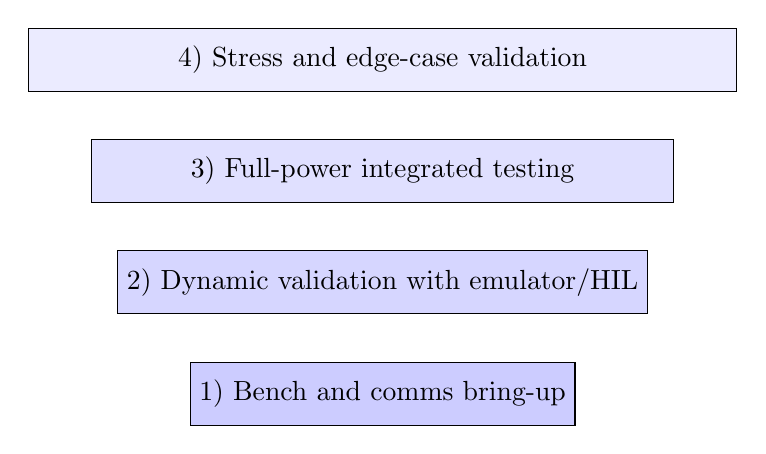
\begin{tikzpicture}[node distance=0.6cm,>=Latex]
  \node[draw,fill=blue!8,minimum width=9cm,minimum height=0.8cm] (a) {4) Stress and edge-case validation};
  \node[draw,fill=blue!12,minimum width=7.4cm,minimum height=0.8cm,below=of a] (b) {3) Full-power integrated testing};
  \node[draw,fill=blue!16,minimum width=5.8cm,minimum height=0.8cm,below=of b] (c) {2) Dynamic validation with emulator/HIL};
  \node[draw,fill=blue!20,minimum width=4.2cm,minimum height=0.8cm,below=of c] (d) {1) Bench and comms bring-up};
\end{tikzpicture}
\end{center}

\subsection{LVRT test skeleton}
\begin{itemize}
  \item Define dip magnitude and duration matrix (for example, \(0.5\pu\) for 0.16 s, \(0.7\pu\) for 0.5 s).
  \item Measure RMS voltage/current, phase angle, DC link behavior, PLL angle/frequency, and trip status.
  \item Verify no nuisance trips inside mandatory ride-through region.
  \item Verify controlled current limiting and post-event recovery without unstable oscillation.
\end{itemize}

\begin{table}[h]
\centering
\begin{tabular}{p{0.21\linewidth}p{0.22\linewidth}p{0.22\linewidth}p{0.25\linewidth}}
\toprule
Test block & Stimulus & Measure & Pass criteria \\
\midrule
Shallow dip & \(0.8\pu\), short duration & Voltage, current, trip flags & No trip and stable synchronization \\
Medium dip & \(0.6\pu\), medium duration & Current limit behavior, control states & Current remains bounded with smooth transition \\
Deep dip & \(0.4\pu\), short duration & Protection sequence timing & Correct ride-through or intentional trip per profile \\
Recovery & Return to nominal voltage & Active/reactive settling behavior & Recovery within target settling time and no retrip \\
\bottomrule
\end{tabular}
\end{table}

\begin{examplebox}{Pass/fail language that sounds senior}
``Pass requires sustained synchronization through all mandatory LVRT points,
bounded current within hardware limits, no protection chatter, and return to
pre-event active power within target settling time without secondary trips.''
\end{examplebox}

\subsection{Instrumentation and data quality expectations}
State clearly that you trust conclusions only if the measurement chain is
credible. Mention calibration status, timestamp alignment, anti-aliasing, and
recording duration long enough to capture pre-event, event, and post-event
dynamics.

\section{Waveform-Centric Troubleshooting Method}

\begin{enumerate}
  \item Reproduce issue with controlled initial conditions.
  \item Build timeline from synchronized data: command, state transition, protection assertion, trip.
  \item Segment by domain: control instability, hardware limit, sensing error, or external grid disturbance.
  \item Test one dominant hypothesis at a time with minimal parameter changes.
  \item Lock in fix with regression test set and field-monitoring hooks.
\end{enumerate}

\begin{table}[h]
\centering
\begin{tabular}{p{0.24\linewidth}p{0.31\linewidth}p{0.34\linewidth}}
\toprule
Observed symptom & Most likely domain & First discriminating test \\
\midrule
Fast current clipping at event start & Hardware limit or current-limit transition & Compare commanded versus measured current with high-speed capture \\
Low-frequency oscillation after setpoint step & Control-loop interaction & Reduce one loop bandwidth and repeat identical step test \\
Intermittent trip with clean waveforms & Sensing or communications path & Validate data freshness, timeout behavior, and sensor validity flags \\
Site-specific instability only & Grid interaction or plant-level control conflict & Replay site impedance and controller settings in lab emulator \\
\bottomrule
\end{tabular}
\end{table}

\begin{warningbox}{Common integration failure patterns}
\begin{itemize}
  \item PLL bandwidth too high for weak-grid conditions causing phase hunting.
  \item Reactive support settings conflicting with site voltage-regulator behavior.
  \item Current-limit transitions causing controller windup and delayed recovery.
  \item Protection thresholds tuned for stiff-grid assumptions only.
\end{itemize}
\end{warningbox}

\subsection{RCA closure discipline}
Close the loop by documenting root cause, correction, verification evidence,
and rollback criteria. Interviewers often look for this step because it
distinguishes debugging from full lifecycle ownership.

\section{Standards and Compliance Talking Points}

\subsection{IEEE 1547 and UL 1741 framing}
You do not need to quote every clause. Show you can operationalize standards:
\begin{itemize}
  \item Turn interconnection requirements into a settings matrix and test matrix.
  \item Validate ride-through, voltage/frequency trip settings, and response modes.
  \item Preserve traceability: requirement $\rightarrow$ test procedure $\rightarrow$ waveform evidence $\rightarrow$ report.
\end{itemize}

\begin{table}[h]
\centering
\begin{tabular}{p{0.22\linewidth}p{0.34\linewidth}p{0.35\linewidth}}
\toprule
Compliance area & What to configure & What to verify in test \\
\midrule
Voltage ride-through & Undervoltage and overvoltage thresholds and timers & Correct stay-connected or trip behavior across programmed regions \\
Frequency behavior & Under/overfrequency limits and droop profile & Accurate response and no oscillatory power hunting \\
Reactive support & Volt-var curve points and deadband & Reactive response speed and steady-state accuracy \\
Protection reporting & Event logs and alarms & Time-aligned records that support audit and commissioning review \\
\bottomrule
\end{tabular}
\end{table}

\subsection{Local utility coordination}
Utilities may impose site-specific windows, telemetry, and commissioning tests.
Strong answer pattern:
\begin{itemize}
  \item Confirm utility profile early.
  \item Map deviations from default firmware profiles.
  \item Freeze and version-control final as-built settings.
  \item Align field test scripts to utility witness-test expectations before site mobilization.
\end{itemize}

\section{Industrial Communications: What To Say}

\begin{itemize}
  \item Modbus TCP/RTU: straightforward register access, polling strategy matters for latency and determinism.
  \item CAN: robust for distributed embedded control, requires strict ID and timing discipline.
  \item SunSpec: normalized semantic model over Modbus, improves interoperability and reduces vendor-specific glue logic.
\end{itemize}

\begin{table}[h]
\centering
\begin{tabular}{p{0.2\linewidth}p{0.23\linewidth}p{0.24\linewidth}p{0.24\linewidth}}
\toprule
Protocol & Strength & Limitation & Best use in this role \\
\midrule
Modbus RTU & Simple and widely supported over serial links & Lower throughput and multi-drop timing sensitivity & Commissioning and straightforward field integrations \\
Modbus TCP & Familiar data model with Ethernet transport & Polling design can create non-deterministic latency & Plant controller to inverter supervisory data exchange \\
CAN & Deterministic arbitration and robust bus behavior & Requires disciplined identifier design and bus loading checks & Embedded subsystem coordination and fast status/control signals \\
SunSpec (over Modbus) & Standardized semantic map for energy assets & Coverage depends on vendor implementation completeness & Multi-vendor interoperability and faster integration \\
\bottomrule
\end{tabular}
\end{table}

\begin{answerbox}{Interview answer template}
``I treat communications as part of control-system reliability. I define signal
ownership, data freshness limits, timeout behavior, and safe fallback states,
then I verify behavior under packet loss and delayed telemetry rather than only
nominal conditions.''
\end{answerbox}

\subsection{Minimum communications acceptance tests}
Mention handshake, watchdog timeout behavior, stale-data handling, commanded
setpoint integrity, and recovery behavior after link drop and reconnection.

\section{High-Voltage Safety and NEC-Relevant Awareness}

\begin{itemize}
  \item Demonstrate respect for 400--800 Vac and up to 1500 Vdc hazards.
  \item Mention lockout-tagout discipline, energized-work boundaries, and verified absence of voltage before touch.
  \item Discuss grounding and bonding intent, conductor ampacity, and overcurrent coordination at system level.
  \item Emphasize that safety constraints are design inputs, not post-processing checks.
\end{itemize}

\begin{table}[h]
\centering
\begin{tabular}{p{0.24\linewidth}p{0.3\linewidth}p{0.37\linewidth}}
\toprule
Safety focus & Typical control & Interview language that signals ownership \\
\midrule
Electrical shock hazard & Lockout/tagout and absence-of-voltage verification & ``I do not begin energized troubleshooting until isolation state is verified and documented.'' \\
Arc-flash risk & Boundary control, task planning, appropriate personal protective equipment & ``I design test setup to minimize energized rework and exposure time.'' \\
Grounding and bonding quality & Verified bonding path and grounding strategy & ``I treat grounding as both safety and measurement integrity infrastructure.'' \\
Overcurrent protection & Correct OCPD selection and coordination & ``I check selectivity so nuisance operations do not mask true faults.'' \\
\bottomrule
\end{tabular}
\end{table}

\section{Cross-Functional Influence}

\subsection{Design reviews that prevent late-stage failures}
In a cross-functional review, cover:
\begin{itemize}
  \item Thermal implications of overload and ambient derating.
  \item Mechanical layout impact on cable impedance, EMI, and service access.
  \item Controls/software assumptions for sensor fidelity and command latency.
  \item Manufacturing/service constraints for repeatable commissioning.
\end{itemize}

\subsection{Cross-functional conflict resolution framework}
When tradeoffs conflict, explain your approach:
\begin{enumerate}
  \item Clarify non-negotiables (safety, compliance, hardware limits).
  \item Quantify tradeoff space (performance, schedule, cost, maintainability).
  \item Propose testable compromise with explicit acceptance criteria.
  \item Decide with evidence and document rationale for future programs.
\end{enumerate}

\begin{table}[h]
\centering
\begin{tabular}{p{0.22\linewidth}p{0.3\linewidth}p{0.39\linewidth}}
\toprule
Function & Primary concern & What you should contribute \\
\midrule
Controls engineering & Loop stability and algorithm constraints & Parameter boundaries, field observations, and regression test needs \\
Mechanical and thermal & Enclosure layout and heat rejection margin & Cable routing impact, service access, and thermal derating implications \\
Test engineering & Repeatability and data quality & Test matrix priorities and instrumentation requirements \\
Software and firmware & State-machine behavior and diagnostic visibility & Event taxonomy, fault signatures, and safe fallback requirements \\
\bottomrule
\end{tabular}
\end{table}

\section{Behavioral Questions for This Role}

\subsection{Tell me about a difficult field issue you solved}
Structure using STAR:
\begin{itemize}
  \item Situation: intermittent trips at a specific site condition.
  \item Task: restore uptime without compromising safety or compliance.
  \item Action: synchronized waveform capture, narrowed root cause, parameter retune, regression retest.
  \item Result: stable operation, reduced trip rate, documented playbook for fleet rollout.
\end{itemize}

Add quantification whenever possible:
\begin{itemize}
  \item Mention before/after trip rates, availability changes, mean-time-to-recovery, or number of affected sites.
  \item Name the validation depth used before rollout (lab replay, pilot site, then fleet release).
\end{itemize}

\subsection{How do you work independently on ambiguous problems?}
Answer pattern:
\begin{itemize}
  \item Define measurable success criteria early.
  \item Create ranked hypotheses from highest impact and likelihood.
  \item Time-box experiments and update stakeholders with evidence, not opinions.
  \item Escalate only when constraints block safe progress.
\end{itemize}

\begin{table}[h]
\centering
\begin{tabular}{p{0.24\linewidth}p{0.67\linewidth}}
\toprule
Behavior trait & Evidence statement to use in interview \\
\midrule
Ownership & ``I define technical closure criteria up front and keep a living decision log.'' \\
Prioritization & ``I run highest-likelihood, highest-impact hypotheses first and time-box dead ends.'' \\
Communication & ``I send concise evidence updates with explicit ask, risk, and next step.'' \\
Learning loop & ``After closure, I convert fixes into a regression test so the issue does not recur.'' \\
\bottomrule
\end{tabular}
\end{table}

\section{Likely Interview Questions and Strong Responses}

\begin{answerbox}{Q1: How would you tune an inverter for weak-grid stability?}
I would first estimate grid strength (SCR and impedance profile), then set a
conservative baseline: reduced PLL bandwidth for GFL or damped droop/virtual
impedance for GFM. I would validate with step changes in voltage and power,
watch for low-frequency oscillation and current saturation, then iterate one
loop at a time while preserving protection margins.
\end{answerbox}

\begin{answerbox}{Q2: What does a good LVRT validation campaign look like?}
A good campaign uses a parameterized dip matrix, synchronized high-resolution
waveform capture, and explicit pass/fail limits for ride-through, current
envelope, and recovery. It includes pre-checks, repeatability runs, and a
regression subset after any firmware or settings change.
\end{answerbox}

\begin{answerbox}{Q3: How do you separate hardware versus controls root cause?}
I split evidence by timescale and signatures: instantaneous clipping or thermal
foldback suggests hardware limits; oscillatory behavior tied to loop dynamics
points to controls; discontinuities with clean power path can indicate sensing
or comms artifacts. I design A/B tests that isolate one domain at a time.
\end{answerbox}

\begin{answerbox}{Q4: How do you decide between two inverters with similar ratings?}
I compare them on control maturity, diagnostics depth, utility-compliance
flexibility, and support responsiveness, not only on nameplate power. If two
devices have similar \(\kVA\), I prioritize the one that reduces lifecycle risk
through better logging, better weak-grid behavior, and faster field-service
closure.
\end{answerbox}

\begin{answerbox}{Q5: What is your approach when lab and field behavior differ?}
I first normalize assumptions: grid impedance, site controller behavior,
instrumentation fidelity, and firmware versions. Then I recreate the field
condition in emulator or HIL, isolate the deltas, and release corrective changes
with a validation package that explicitly includes both lab replay and field
acceptance checks.
\end{answerbox}

\section{30-60-90 Day Plan You Can Present}

\begin{longtable}{p{0.18\linewidth}p{0.76\linewidth}}
\toprule
Window & Proposed Impact \\
\midrule
0--30 days & Learn platform architecture, inverter vendor capabilities, site profiles, and safety workflows. Build baseline test scripts and reproduce one known issue in the lab. \\
31--60 days & Own a complete validation plan for one integration release, including LVRT and frequency response. Deliver first settings recommendation package with traceable evidence. \\
61--90 days & Lead root-cause closure for one field issue end-to-end, formalize regression suite, and publish a cross-functional integration checklist used by test, controls, and field teams. \\
\bottomrule
\end{longtable}

\subsection{Milestones and measurable indicators}
\begin{table}[h]
\centering
\begin{tabular}{p{0.2\linewidth}p{0.23\linewidth}p{0.48\linewidth}}
\toprule
Window & Milestone & Evidence of success \\
\midrule
0--30 days & Technical onboarding complete & Can independently run baseline tests and explain controls/protection architecture \\
31--60 days & First integration recommendation delivered & Signed-off test report with traceable settings rationale \\
61--90 days & First field issue closed & RCA, corrective validation, and regression test integrated into team process \\
\bottomrule
\end{tabular}
\end{table}

\section{Final Day-Before Interview Checklist}

\begin{itemize}
  \item Prepare two deep technical stories: one lab characterization, one field RCA.
  \item Review IEEE 1547 function categories and practical implications for settings.
  \item Rehearse a concise explanation of GFL versus GFM and when each fails.
  \item Be ready to draw a waveform timeline and explain trip causality.
  \item Prepare one question each for controls, test engineering, and field operations.
\end{itemize}

\subsection{Rapid rehearsal script}
Use a 10-minute prep cycle:
\begin{enumerate}
  \item Two-minute role summary: who you are and where you create value.
  \item Three-minute deep dive: one LVRT or weak-grid tuning story.
  \item Three-minute field RCA story with measurable impact.
  \item Two-minute close: why this role and what you will deliver in 90 days.
\end{enumerate}

\begin{keybox}{Close strong}
``I am most effective where power electronics, controls, and real-world grid
conditions meet. I can own that interface from architecture through validation
and field reliability with a safety-first and evidence-first mindset.''
\end{keybox}

\end{document}
